\documentclass{article}
\usepackage[utf8]{inputenc}
\usepackage{babel}
\usepackage{polski}
\usepackage{float}
\title{Wykład 1}
\maketitle
\begin{document}

	\section{Analiza wielowymiarowego obiektu sterowania w przestrzeni stanu}

	\subsection{Definicja obiektu sterowania}
		\begin{itemize}
			\item Obiekt nazywamy obiektem sterowania gdy sterownik/podmiot sterujący oddziaływuje
			na dynamikę ewolucji stanu obiektu.
			\item Skutki tych działań obserwujemy przez sygnały wyjściowe
			\item Wielowymiarowy obiekt sterowania to taki obiekt który ma wiele wejść,
			oraz wiele wyjść.
			\item Wystarczy że liczba sygnałów sterujących, sygnałów zakłócających bądź sygnałów
			wyjściowych będzie większa od 1 aby była mowa o obiekcie wielowymiarowym
			\item Nazywamy go obiektem MIMO, czyli Multiple Input Multiple Output
		\end{itemize}
	\subsection{Rodzaje sygnałów wejściowych}

		Sygnały wejściowe dzielimy na sygnały sterujące oraz sygnały zakłócające.

		Sygnały sterujące to takie sygnały, które możemy modulować aby osiągnąc cel sterowania.
		Tym celem może być na przykład uzyskanie danego przebiegu zmiennych stanu obiektu

		Pozostałe sygnały traktujemy jak sygnały zakłócające. Reprezentują one oddziaływanie
		czynników środowiskowych na obiekt sterowania. Nie możemy na przebieg tych
		sygnały wpływać, ale zazwyczaj możemy je zmierzyć

	\subsection{Analiza obiektu sterowania typu MIMO}

	Analiza obiektów MIMO znacząco różni sie od obiektów SISO poznanych wcześniej.
	Wynika to z tego, że trzeba uwzględnić interakcje sygnałów pomiędzy sobą.
	Takie interakcje nazywamy również sprzężeniami skrośnymi w strukturze obiektu

	Ta nazwa będzie mieć więcej sensu później, na razie zapamiętaj że ona się pojawiła

	Każdy sygnał sterujący ma potencjał aby wpływał na pozostałe sygnały wyjściowe.
	Konsekwencją tego jest to że nie możemy po prostu zwiększyć liczby podproblemów
	typu Single Input Single Output. Dobranie regulatora do obiektu MIMO komplikuje
	właśnie przez to że sygnały są współzależne od siebie.

	\section{Sporządzanie modeli MIMO w przestrzeni stanu}

	\subsection{Podejście eksperymentalne}

		Podejście eksperymentalne będzie również nazywane eksperymentem w dalszej
		części opracowania

		Podejście eksperymentalne polega na oddzielnym pobudzaniu sygnałem harmonicznym
		(np sinusoidom) o znanej pulsacji wejść obiektu. Celem tego jest wyznaczenie w
		stanie ustalonym wzmocnień oraz przesunięć fazowych, a następnie zapisanie
		charakterystyk amplitudowo fazowych poszczególnych kanałów przepływu sygnału.

		Podejście to sprawdza się tylko w wyjątkowych przypadkach
		do sporządzenia modelu wejść-wyjść obiektu.
		Taki przypadek następuje gdy badany obiekt jest stabilnym liniowo
		obiektem niskiego rzędu.

	\subsection{Przepływ sygnałów w systemach złożonych}

		Przez kanał rozumiemy scieżkę jaką przeszedł sygnał od danego wejścia
		do danego wyjścia obiektu. Tą ścieżkę łatwo sobie zwizualizować na
		Grafie Sygnałowym Masona
		\begin{figure}
			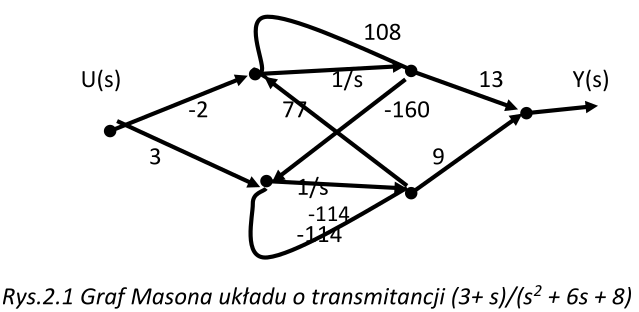
\includegraphics{GrafMasona.png}
		\end{figure}
		Taki graf może pomóc nam rozrysować połączenie dowolnie obranego wejścia z
		dowolnie obranym wyjściem. Jak widać takie połączenie możemy opisać transmitancją.
		Nie dla każdego połączenia wejścia oraz wyjścia istnieje połączenie, wówczas taki
		kanał nie istnieje, a transmitancja jest równa zero.

	\subsection{Sporządzanie właściwego modelu obiektu w przestrzeni stanu}

		W wyniku eksperymentalnego podejścia opisanego wyżej otrzymujemy jedynie dyskretne
		punkty charakterystyki amplitudowo-fazowej. Przebieg charakterystyki dla
		wszystkich możliwych pulsacji otrzymujemy za pomocą aproksymacji np.
		metodą najmniejszych kwadratów.

		Aproksymacja ta jest zadaniem stosunkowo prostym jedynie dla kanałów
		charakteryzujących się dynamika niskiego rzędu.
		Czyli takich gdzie mianownik transmitancji widmowej jest niskiego rzędu,
		a licznik jest rzędu nie większego od rzędu mianownika.
		Najprościej jest gdy licznik nigdy się nie zeruje.
		Można również się posłużyć krzywikiem lub matlabem.
		(przyp. tł. nie wiem czym jest krzywik i szczerze mówiąc chuj mnie to obchodzi)

		Dla dynamiki niskiego rzędu mniejszych od 4 istnieją stabelaryzowane charakterystyki
		modelowe, które porównujemy z rezultatem aproksymacji na zasadzie graficznego
		podobieństwa. Takie stwierdzenie podobieństwa upoważnia nas do podporządkowania
		charakterystyki do jednej z klas modelowych.
		Klasy te mają określoną ogólną postać parametryczną $G(s)$ oraz $G(\omega j)$.
		Dane transmitancje z tabeli mają posiadają sparametryzowane niektóre parametry.
		Tymi parametrami mogą być
		\begin{itemize}
			\item współczynnik wzmocnienia
			\item stałe czasowe
			\item tłumienność
			\item okres drgań własnych
		\end{itemize}
		Dysponując konkretnym przebiegiem charakterystyki amplitudowo-fazowej możemy przystąpić
		do wyznaczania nieznanych parametrów. Parametry można wyznaczyć
		\begin{itemize}
			\item graficznie. Jednak każda modelowa charakterystyka posiada specyficzny sposób wyznaczania
			tych parametrów
			\item analitycznie, rozwiązując układ równań. Po lewej stronie równania wpisujemy
			wyznaczone z eksperymentu moduły i fazy, natomiast po prawej stronie wstawiamy
			sparametryzowane wartości z transmitancji z tabelki. Za $\omega j$ wstawiamy
			konkretne wartości dla których był przeprowadzany eksperyment.
		\end{itemize}
	\subsection{Konsekwencje otrzymanego modelu stanu}

		Sukces powyższej metody w dużej mierze zależy od możliwie najmniejszej ilości
		szumów w układzie oraz szumów pomiarowych. Rezultatem żmudnego eksperymentu
		jest niesparametryzowana postać obiektu sterowania w postaci dyskretnych tablic
		próbek charakterystyk amplitudowo-fazowych poszczególnych kanałów wejścia-wyjścia.
		Tablice te są w postaci pary modułu oraz przesunięcia fazowego, dla danej pulsacji
		pobudzenia.

		Otrzymane transmitancje dla poszczególnych wejść oraz wyjść następnie możemy
		wsadzić do macierzy dumnie nazywającą się transmitancją macierzową
		wielowymiarowego obiektu sterowania

		Elementy na przekątnej reprezentują transmitancje własne kanałów
		wejścia-wyjścia, natomiast elementy poza diagonalą to są
		wcześniej wspomniane transmitancje skrośne. Jeśli dany kanał wejścia nie jest
		połączony z innym kanałem wyjścia to w tym miejscu gdzie powinna być
		transmitancja danego wejścia wyjścia macierz posiada wartość zero.

		Ta macierz może być punktem wyjścia do wyprowadzenia równań w dziedzinie czasu,
		wiążących poszczególne sygnały wyjściowe z poszczególnymi sygnałami wejściowymi albowiem:
		\begin{equation}
			 M_{ij}(s) \cdot Y_{j}(s) = L_{ij}(s) \cdot U_{i}(s) 
		\end{equation}
		Gdzie M jest mianownikiem transmitancji a L jest licznikiem.
		i oraz j oznaczają kolejno numer wejścia oraz numer wyjścia.

		Stosując odwrotną transformatę Laplace'a otrzymujemy równania różniczkowe w
		dziedzinie czasu.

		\begin{equation}
			y^{(n)}(t) + a_{n-1} y^{(n-1)}(t) + ... +   a_{0} y(t) = b_{(m)} u(t) + ... + b_{0} u(t)
		\end{equation}
		Najczęściej mamy do czynienia z przypadkami, gdy w poszczególnych
		transmitancjach G_{ij}(s) nie występują zera.
		Wtedy taki kanał ma statyczny współczynnik wzmocnienia k_{ij} = b_{0 ij}

		Postać ogólną równania otrzymujemy rozwiązaując równanie jednorodne
		\begin{equation}
			y^{(n)}(t) + a_{n-1} y^{(n-1)}(t) + ... +   a_{0} y(t) = 0
		\end{equation}
		Ponieważ jest to równanie liniowe n-tego rzędu, to jego rozwiązanie wymaga znajomości
		n warunków początkowych

		Dla każdego z sygnałów wyjściowych należy ustalić maksymalny rząd jego
		pochodnej względem czasu. Pochodne te znajdujemy przeglądając wierszami
		transmitancje macierzową.
		(przyp. tł. ostatni paragraf jest zlepkiem informacji bez wzniosków bo te
		są zawarte w następnej prezentacji)
\end{document}

